  \label{ex:recursivetranspose}
  Implement a recursive algorithm for matrix transposition:

  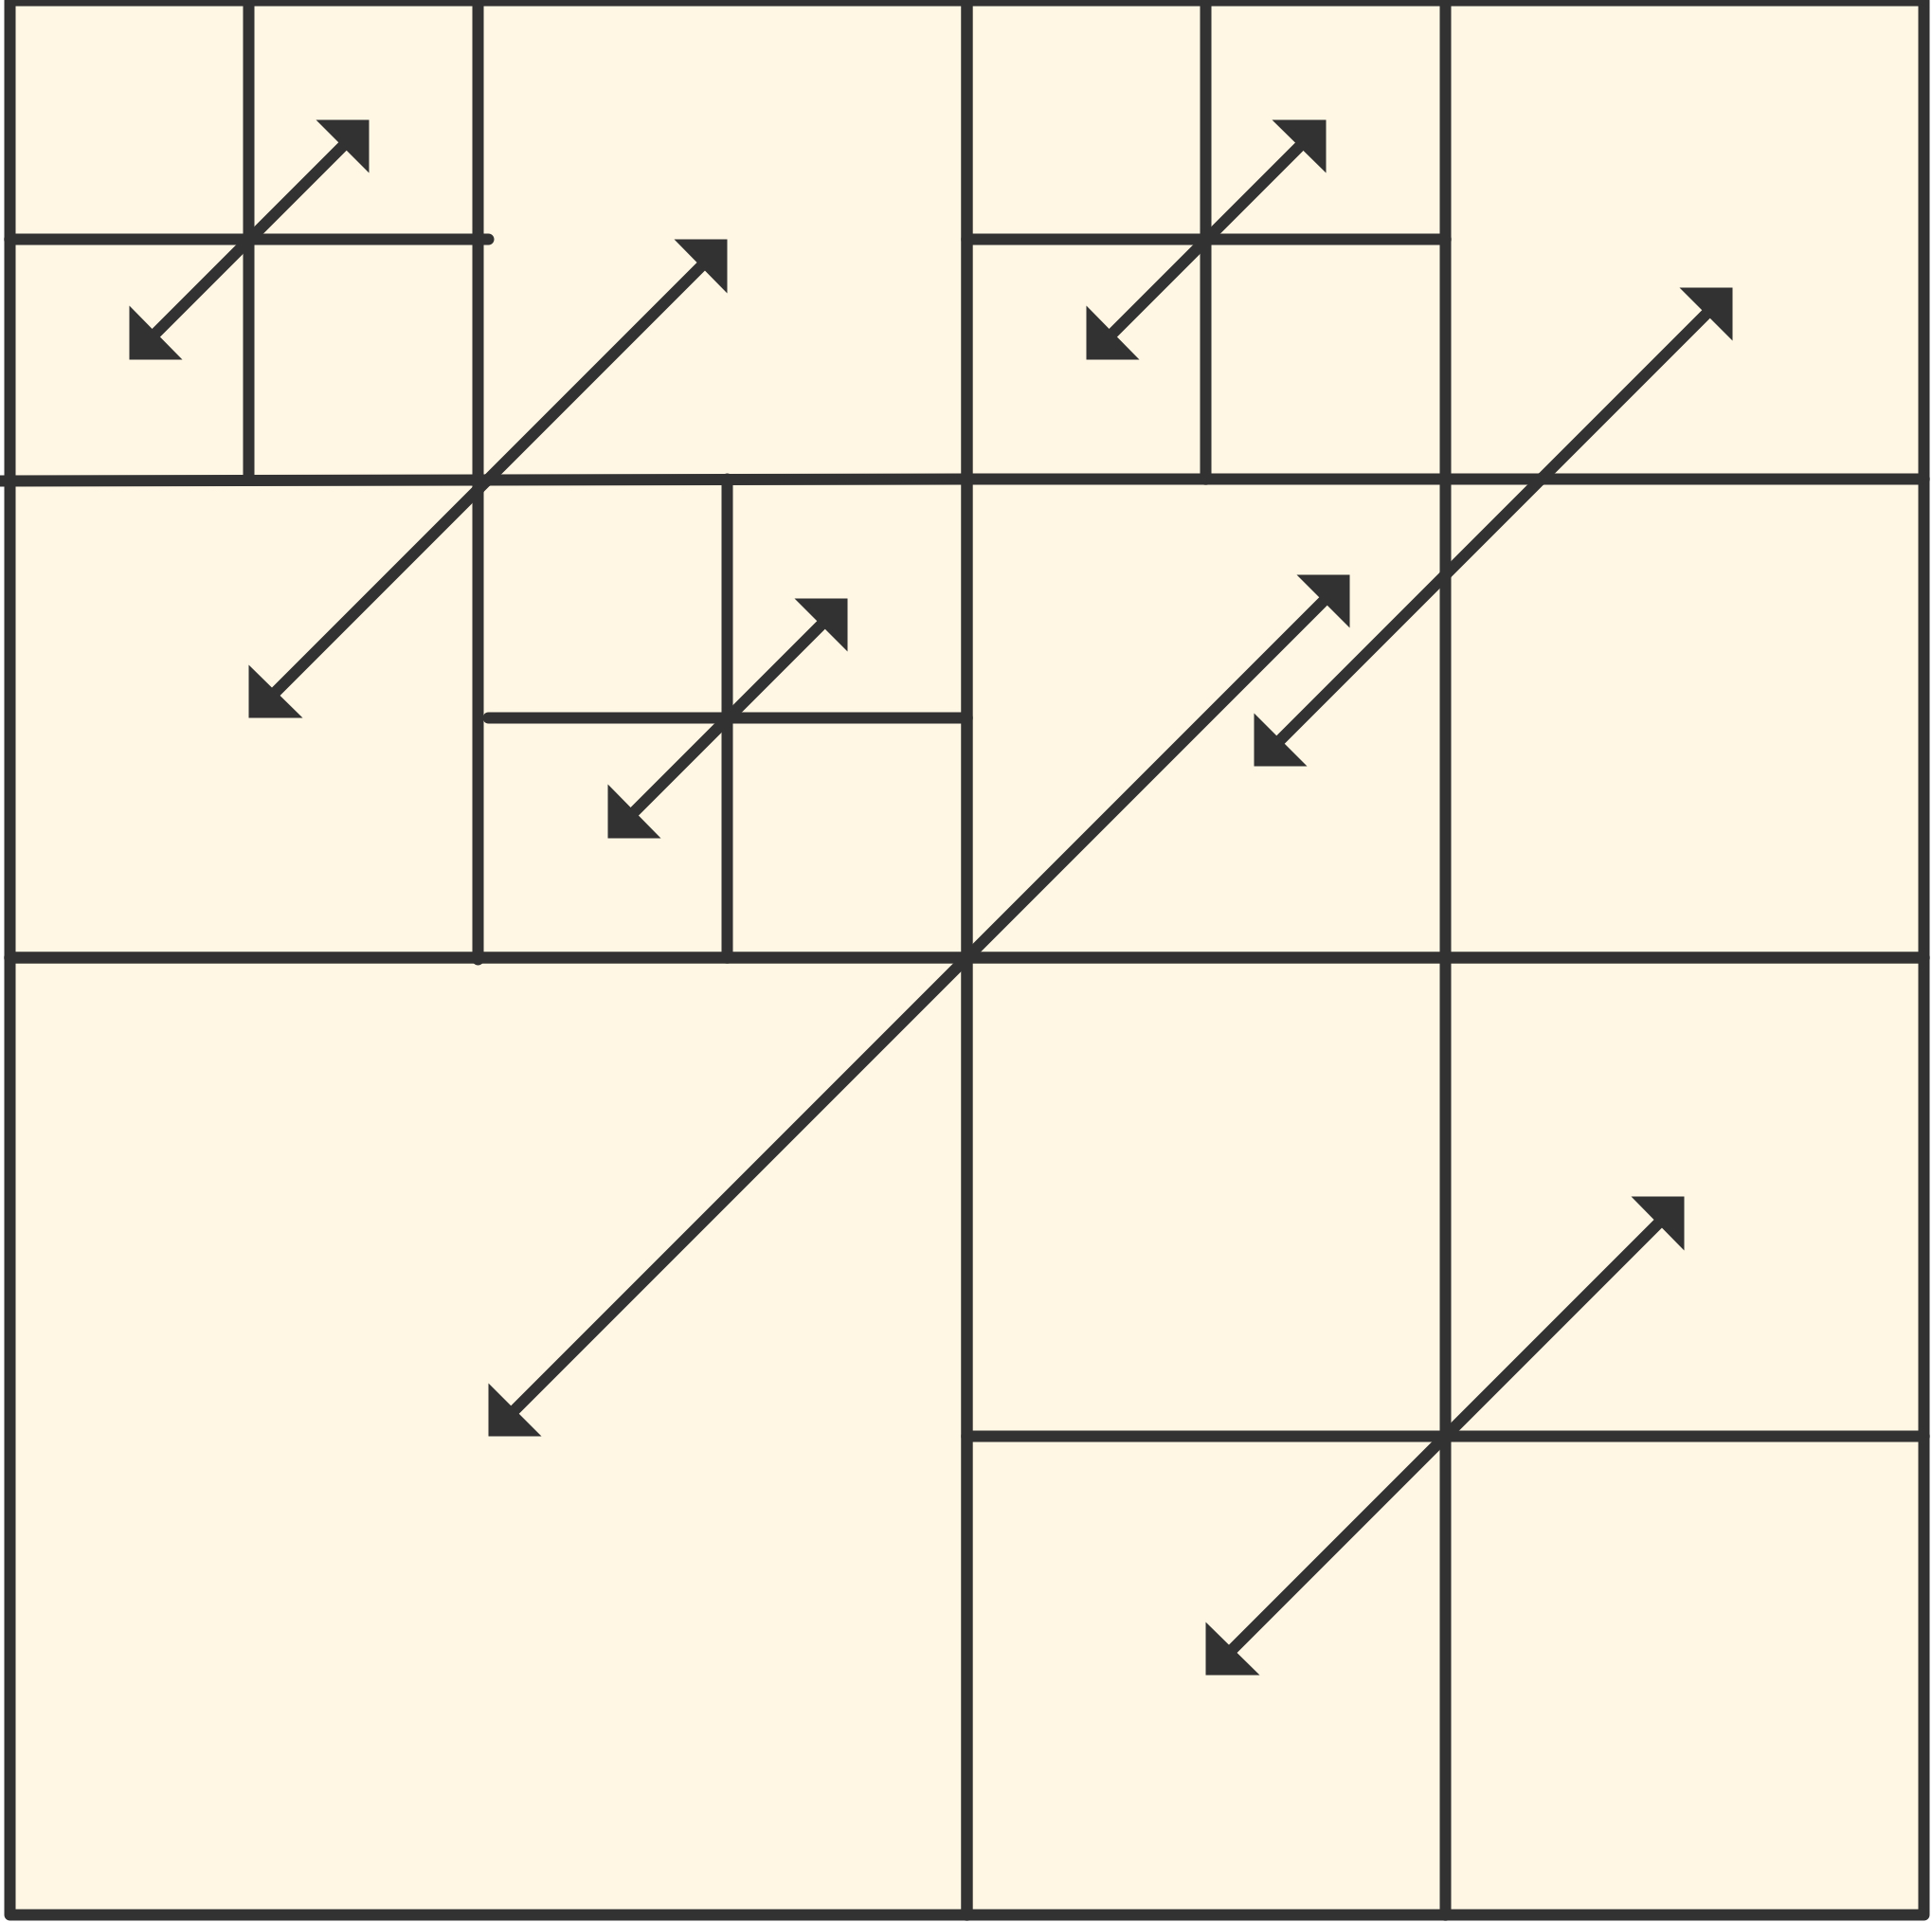
\includegraphics[scale=.1]{recursive-transpose}

  \begin{itemize}
  \item Swap blocks $(1,2)$ and $(2,1)$; then
  \item Divide the processors into four subcommunicators, and
    apply this algorithm recursively on each;
  \item If the communicator has only one process, transpose the matrix in place.
  \end{itemize}
